\documentclass[a4paper,12pt]{article}

\usepackage{cmap}					
\usepackage[T2A]{fontenc}
\usepackage[utf8]{inputenc}
\usepackage[english,russian]{babel}
\usepackage{hyperref}
\usepackage{graphicx}

\hypersetup{
    colorlinks=true,
    linkcolor=blue,
    filecolor=magenta,      
    urlcolor=cyan,
}

\usepackage{amsmath,amsfonts,amssymb,mathtools}
\usepackage{icomma}

\usepackage{euscript}
\usepackage{mathrsfs}
\usepackage{graphicx}
\usepackage{eso-pic}

\graphicspath{ {images/} }

\title{Методы Оптимизации. Лабораторная работа №2}
\author{Раков Николай, Булкина Милена}
\date{}

\begin{document}

\maketitle
\clearpage

\section{Постановка задания}

\begin{enumerate} 
\item Реализовать и протестировать следующие алгоритмы:
\begin{itemize}
\item Метод Градиентного Спуска
\item Метод Наискорейшего Спуска
\item Метод Сопряженных Градиентов
\end{itemize}

\item Оценить, как меняется скорость сходимости, если для поиска величины шага использовать различные методы одномерного поиска.
\item Проанализировать траектории методов для нескольких квадратичных функций.
\item Исследовать, как зависит число итераций от числа обусловленности и размерности пространства.

\end{enumerate}

\section{Анализ траектории методов для квадратичных функций}

Исходная функция
\begin{equation*}
    f(x, y) = 24x^2 + 63y^2 + 56x - 122y + 2
\end{equation*}

Найдём производную по $x_1$ и $x_2$ и приравняем нулю
    \[48x + 56 = 0\]
    \[126y - 122 = 0\]
Получаем, что в (-1.66667, 0.96825) достигается минимум функции.

\clearpage

\subsection{Метод Градиентного Спуска}

В данном методе, чтобы вычислить следующую точку, выбирается направление, обратное градиенту и задается шаг. Значение шага получаем с предыдущей итерации. На каждой следующей итерации мы уменьшаем шаг в два раза до момента, пока значение функции в этой точке после шага не станет меньше текущего.

\begin{center}
    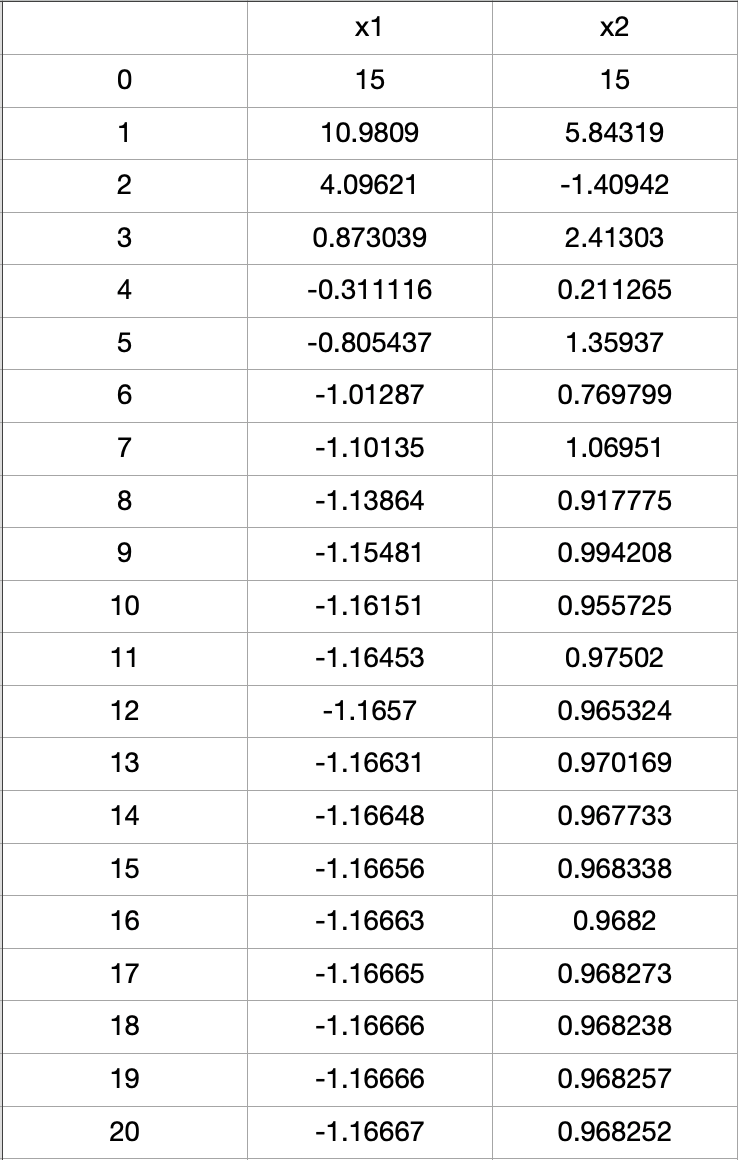
\includegraphics[width=90mm]{table_1.png}

    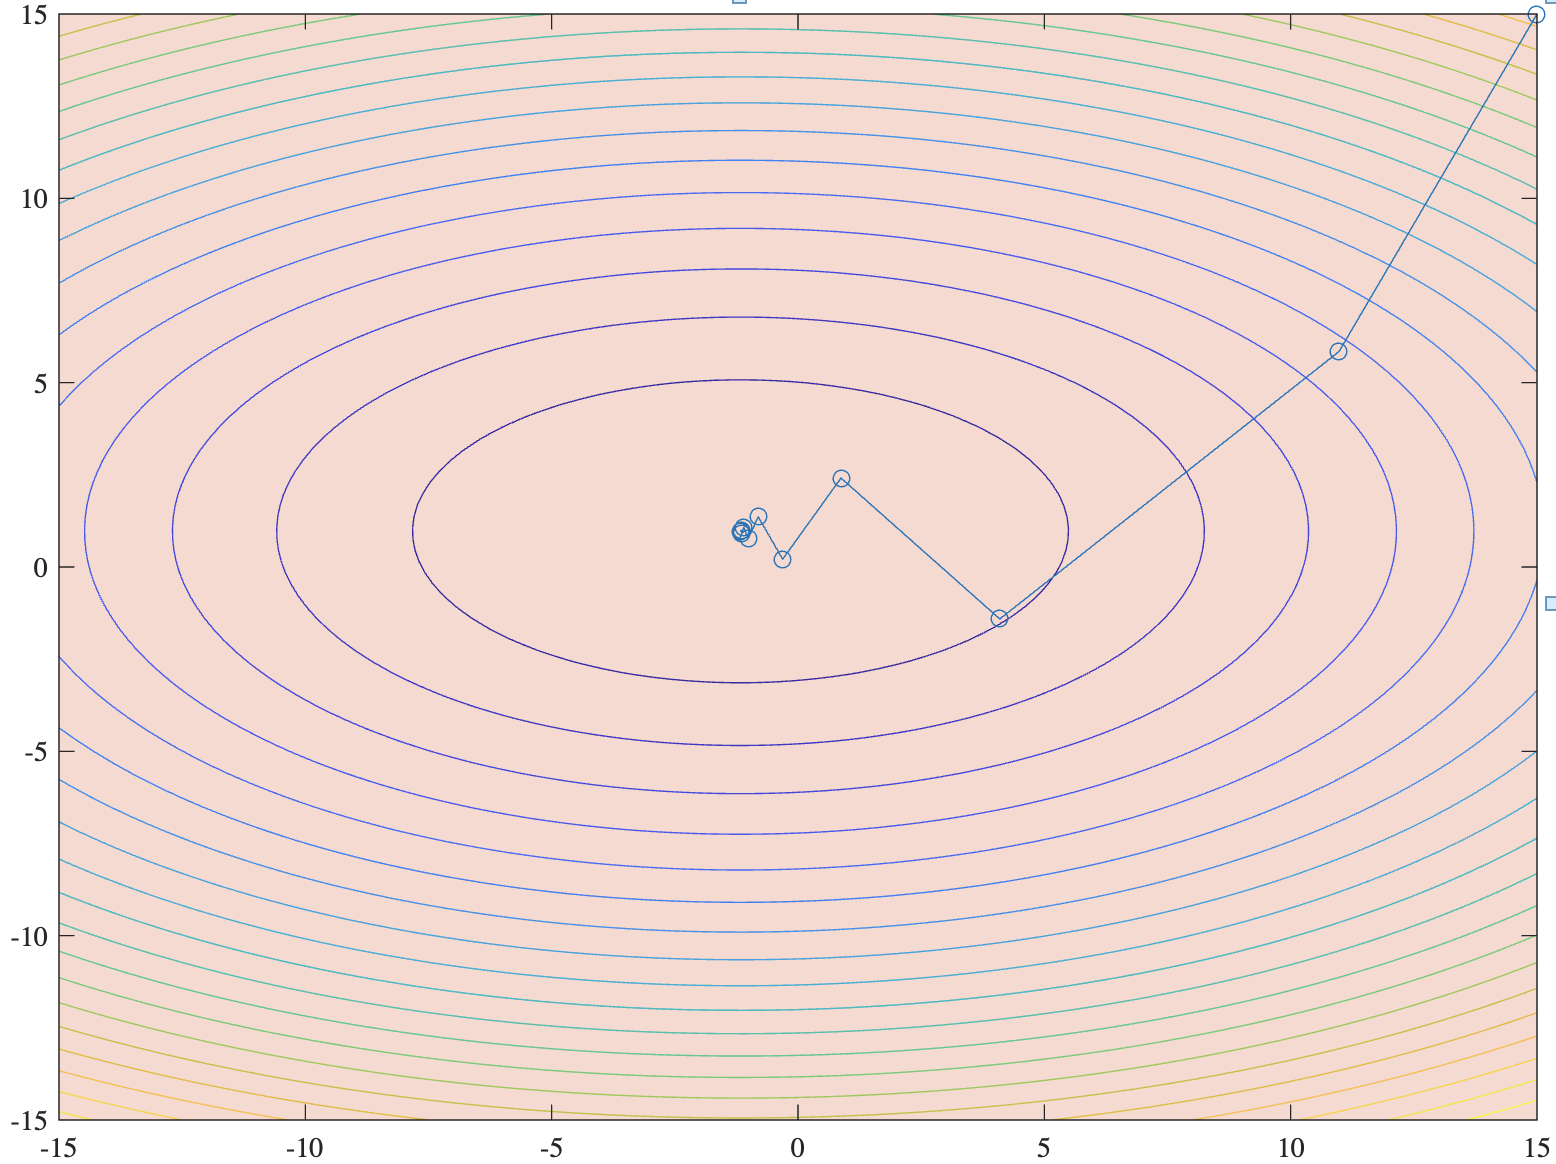
\includegraphics[width=150mm]{plot_1.png}
\end{center}


\clearpage

\subsection{Метод Наискорейшего Спуска}
Метод является улучшением метода градиентного спуска. Делаем шаг в минимум на прямой с направлением градиента. Чтобы найти минимум используется метод одномерной оптимизации.

 \begin{center}
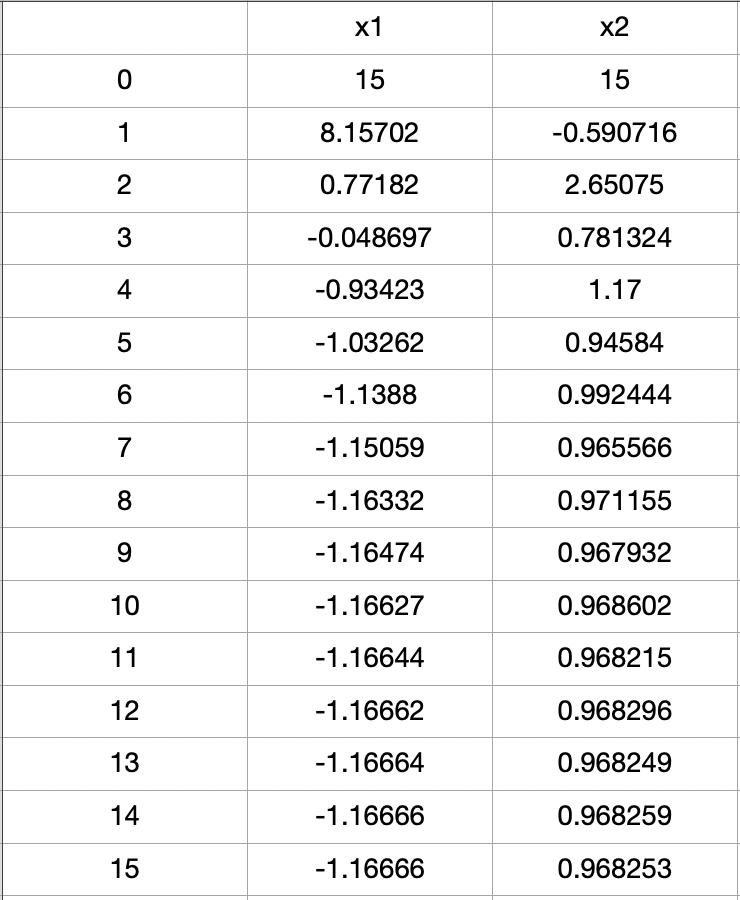
\includegraphics[width=70mm]{table_2.png}

{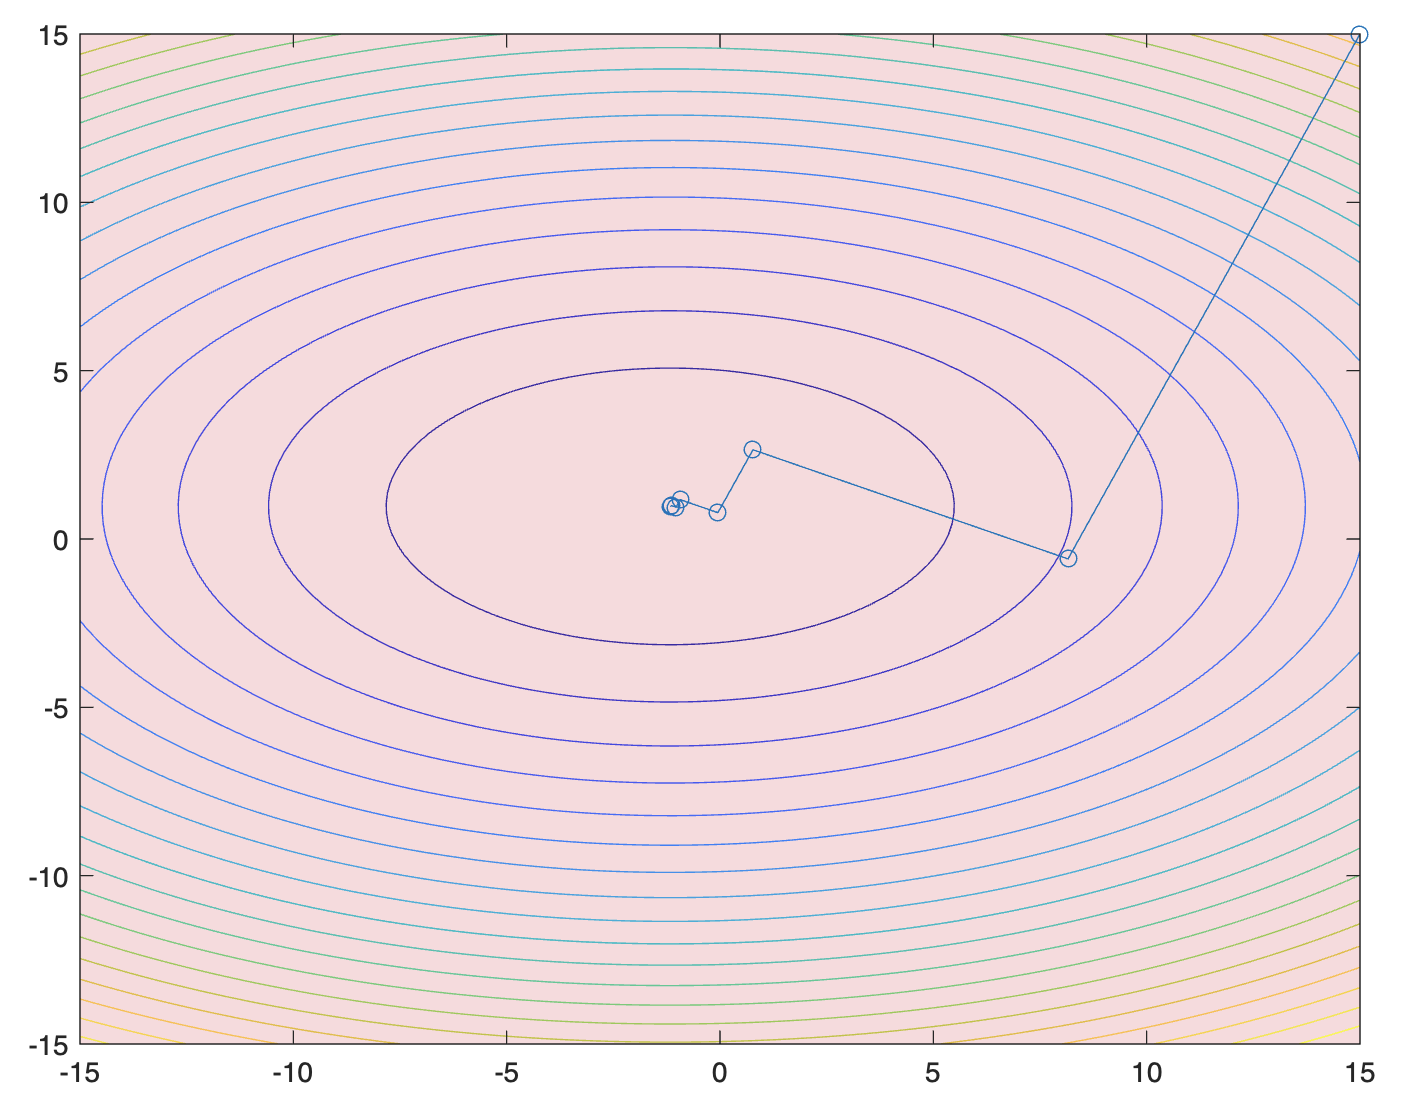
\includegraphics[width=120mm]{plot_2.png}}
 \end{center}

\clearpage

\subsection{Метод Сопряженных Градиентов}

В отличии от двух предыдущих методов, используется не только вектор антиградиета, в методе сопряженных градиентов направления спуска - это A-ортогональные вектора. Из-за этого число итераций не превышает размерность пространства.

\begin{center}
    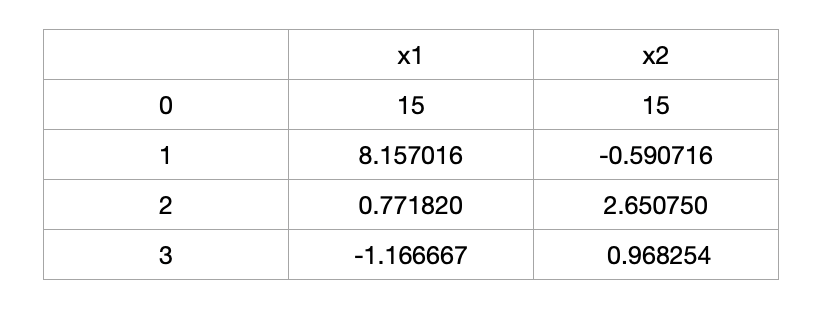
\includegraphics[width=120mm]{table_3.png}
    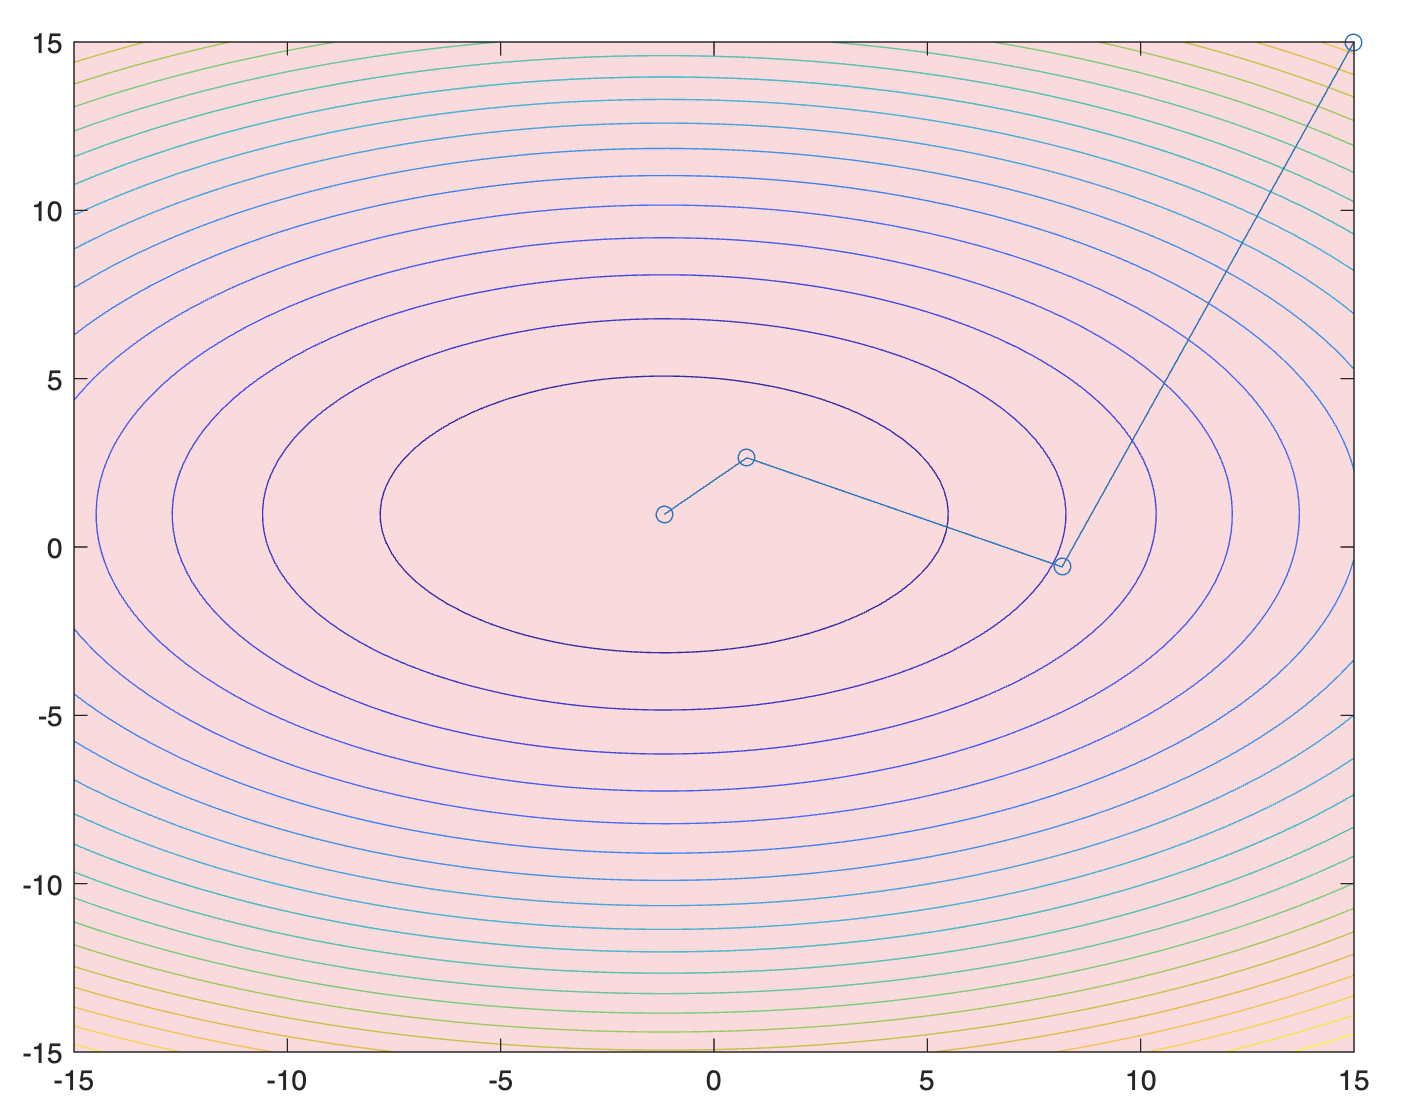
\includegraphics[width=120mm]{plot_3.png}
\end{center}[h]

\clearpage

\section{Траектория методов на различных квадратичных функциях}

\begin{equation*}
    f_1(x, y) = x^2 + 10y^2 - 4x - 4y
\end{equation*}

\begin{center}
    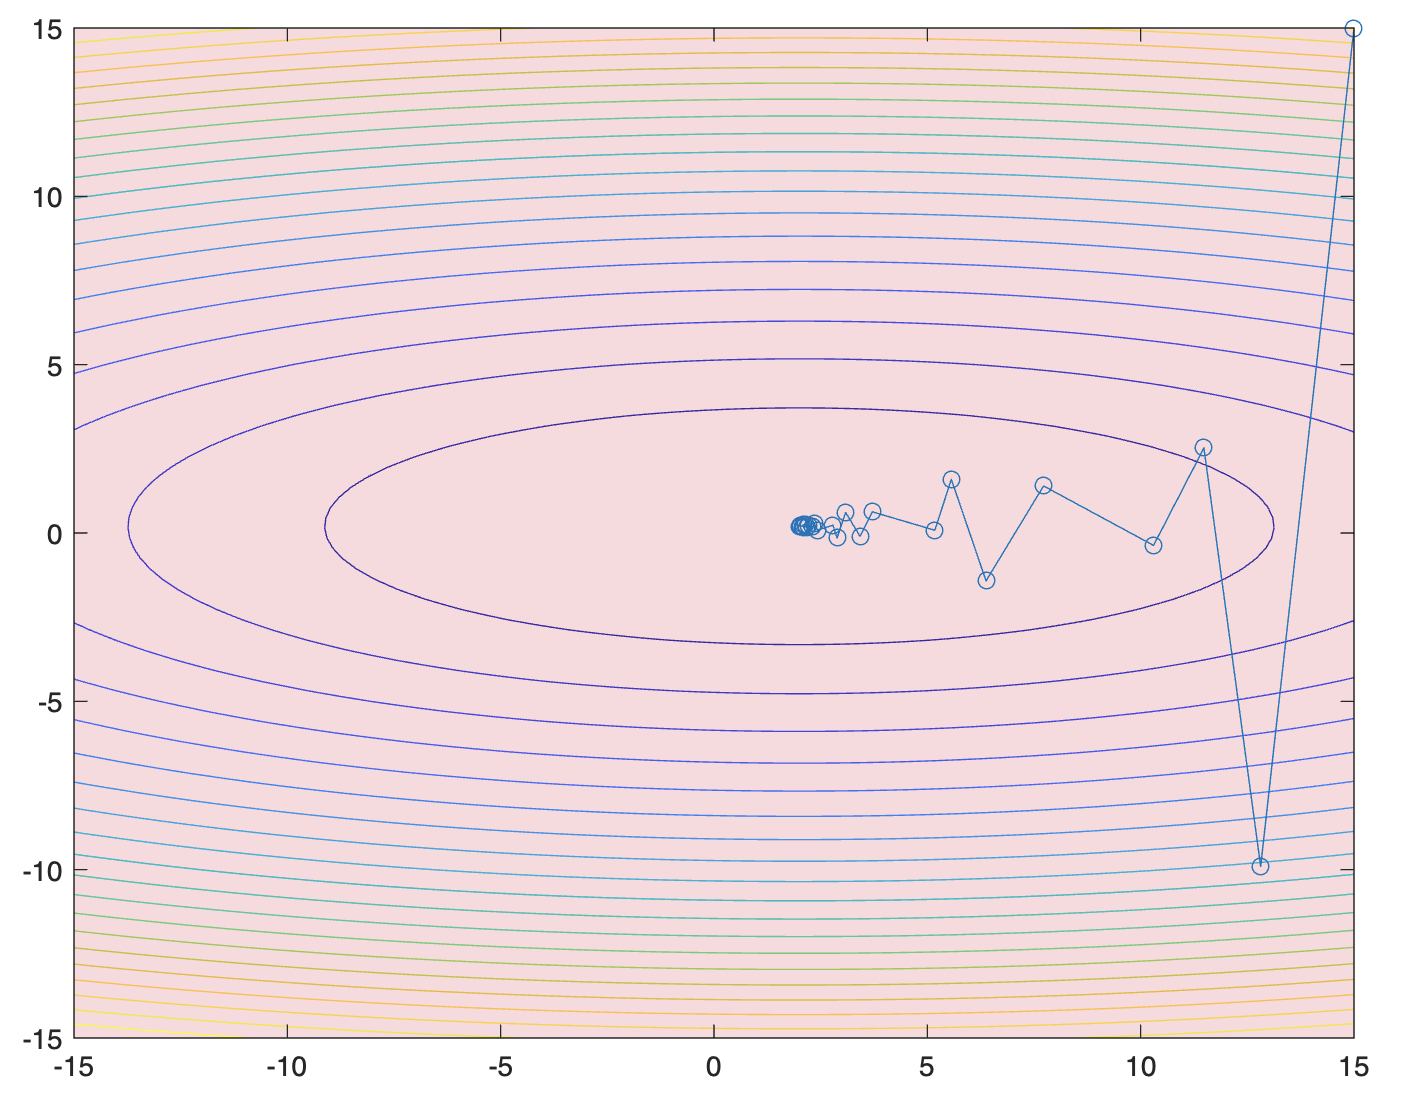
\includegraphics[width=130mm]{p11.png}

    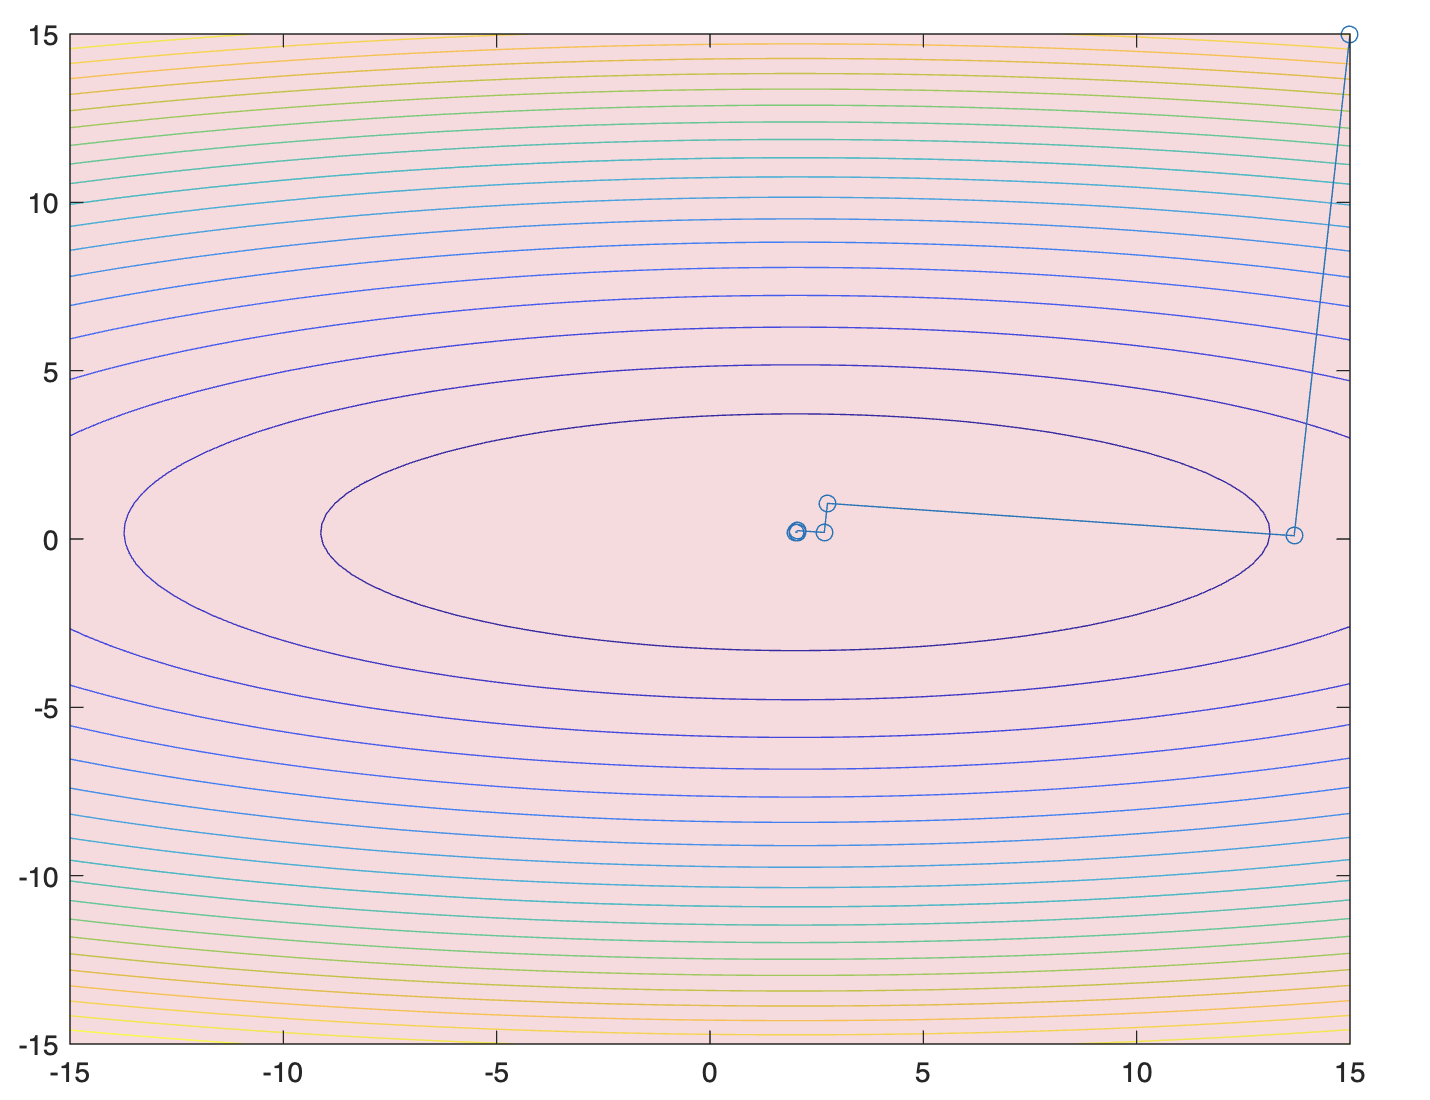
\includegraphics[width=80mm]{p21.png}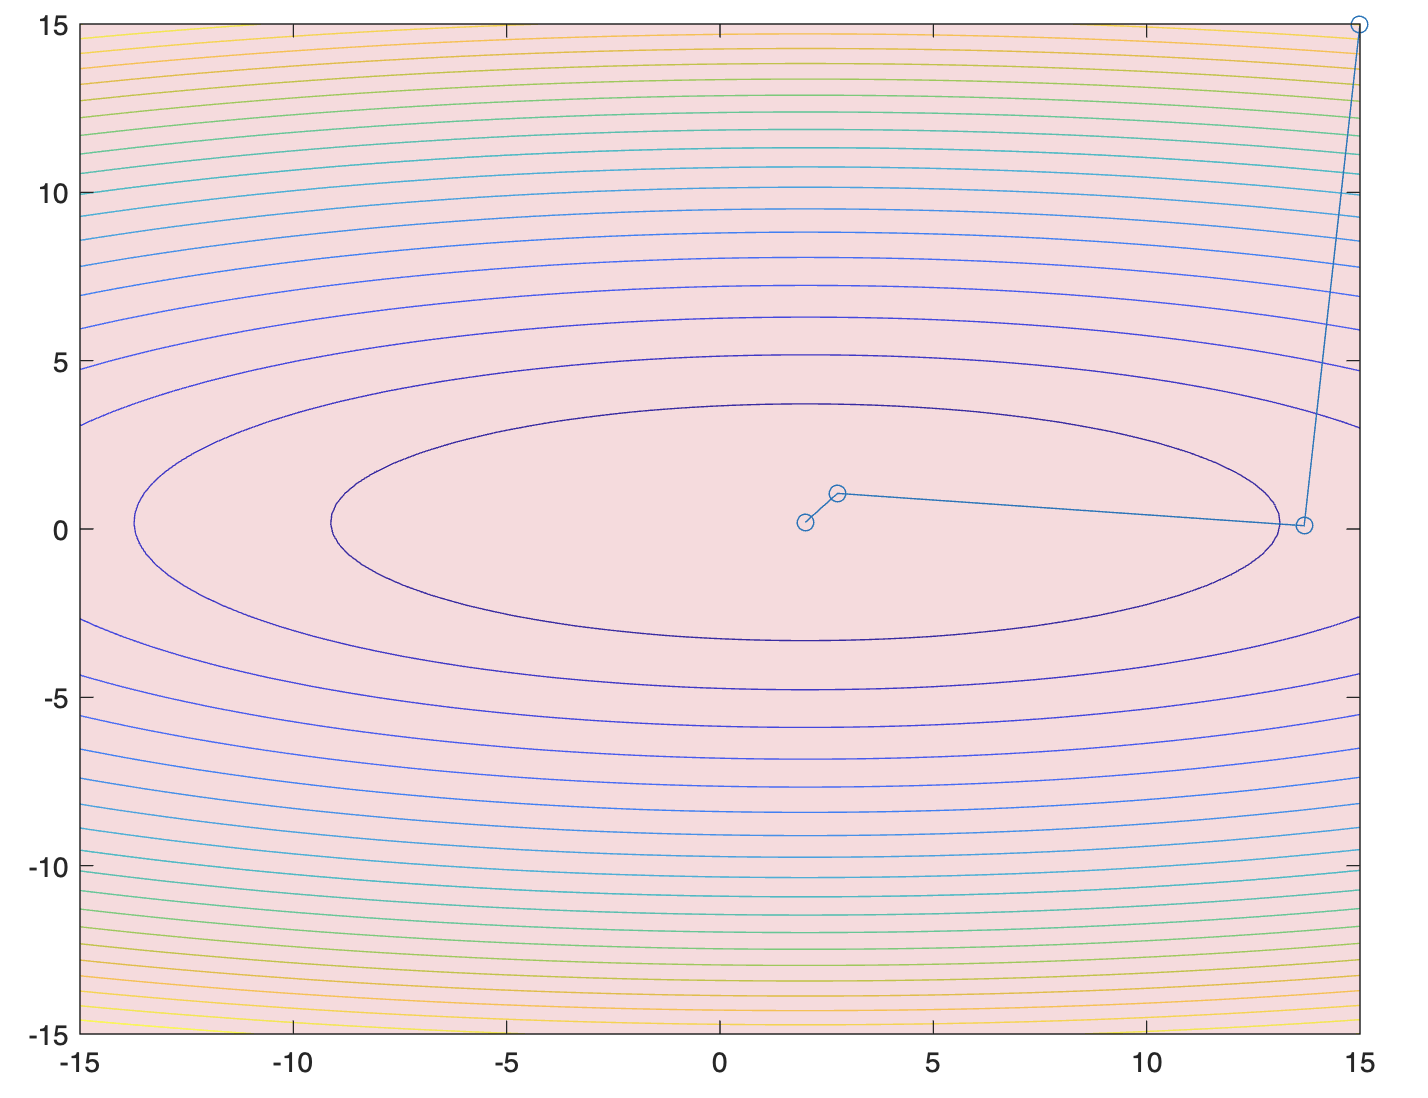
\includegraphics[width=80mm]{p31.png}
\end{center}

\clearpage

\begin{equation*}
    f_2(x, y) = 100x^2 + 2y^2 - 7x - 2y
\end{equation*}

\begin{center}
    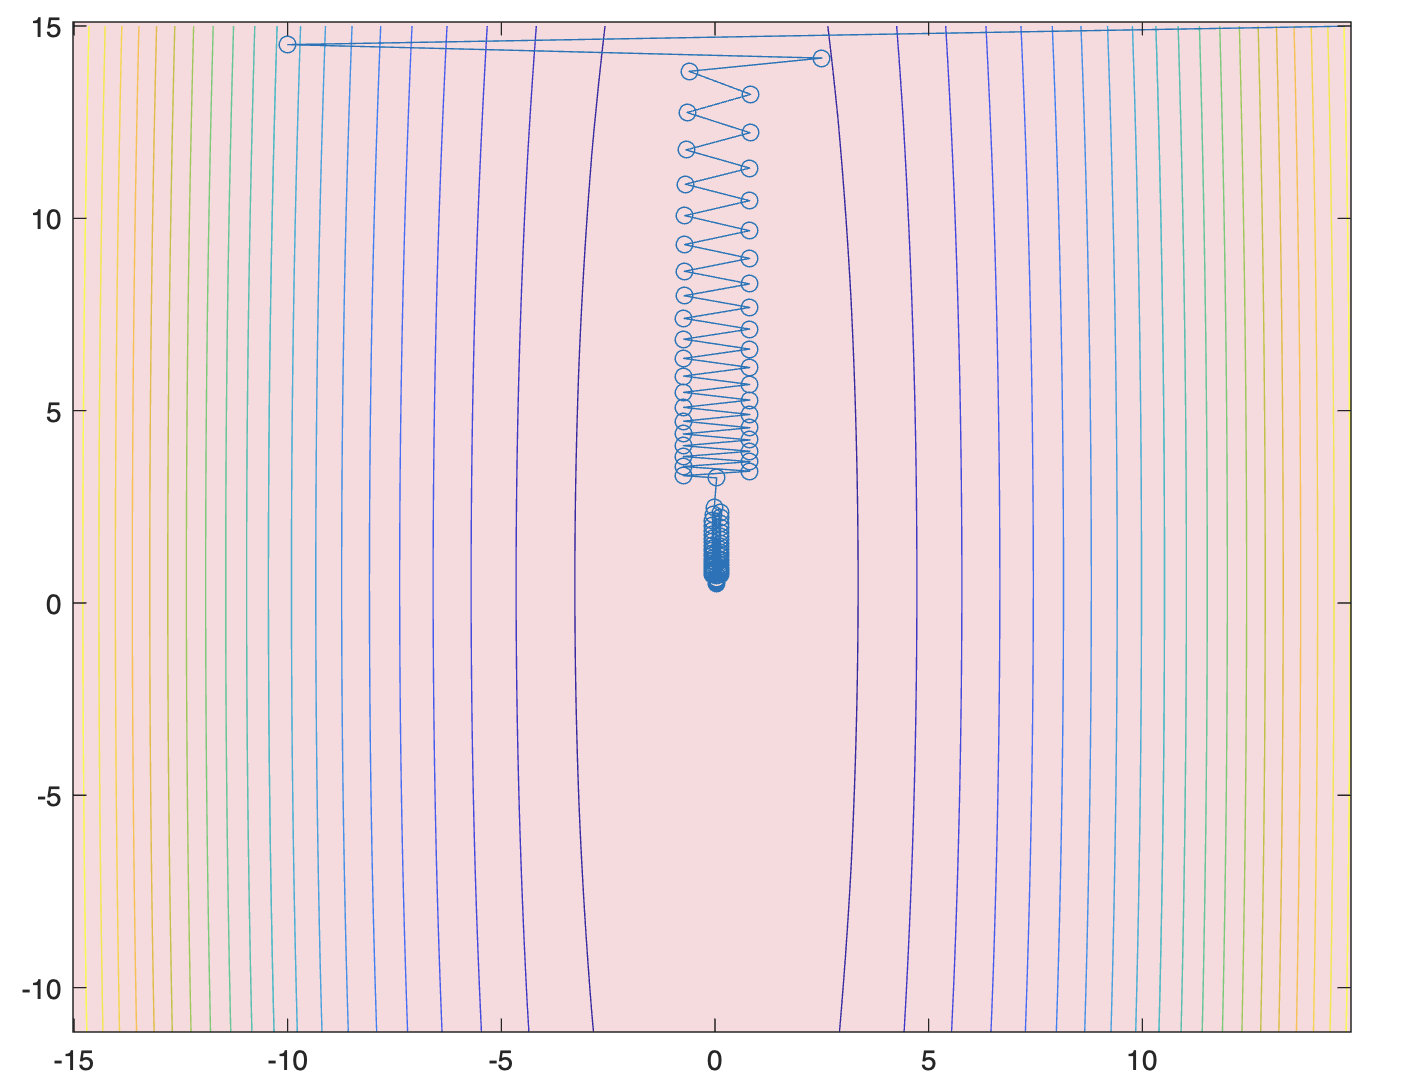
\includegraphics[width=130mm]{p12.png}

    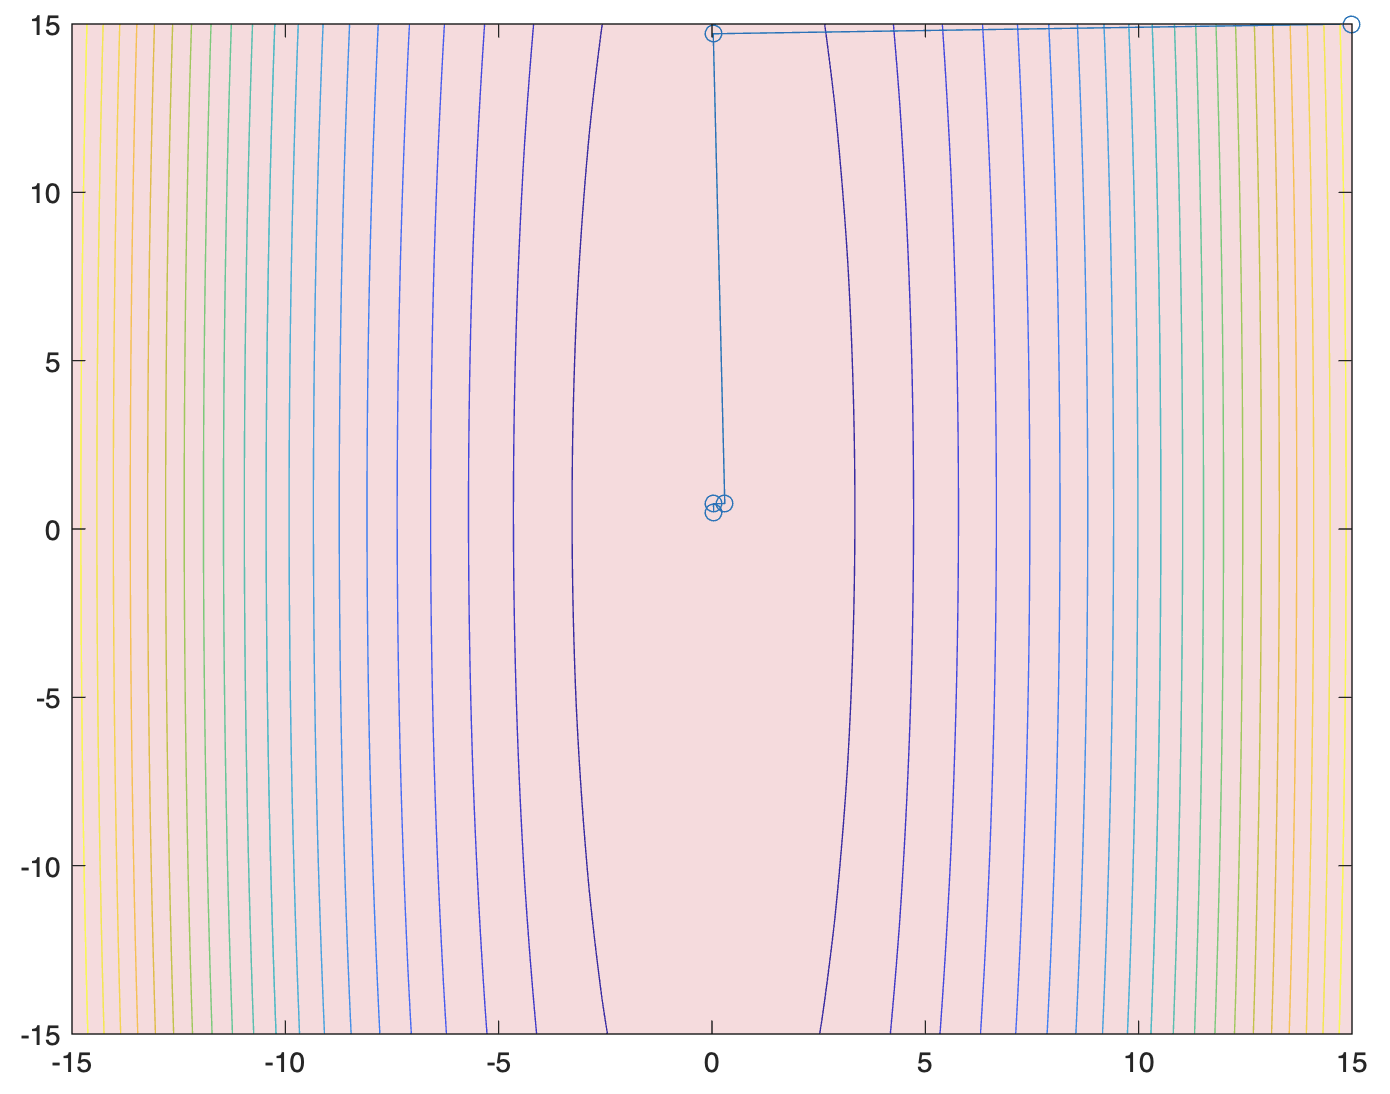
\includegraphics[width=80mm]{p22.png}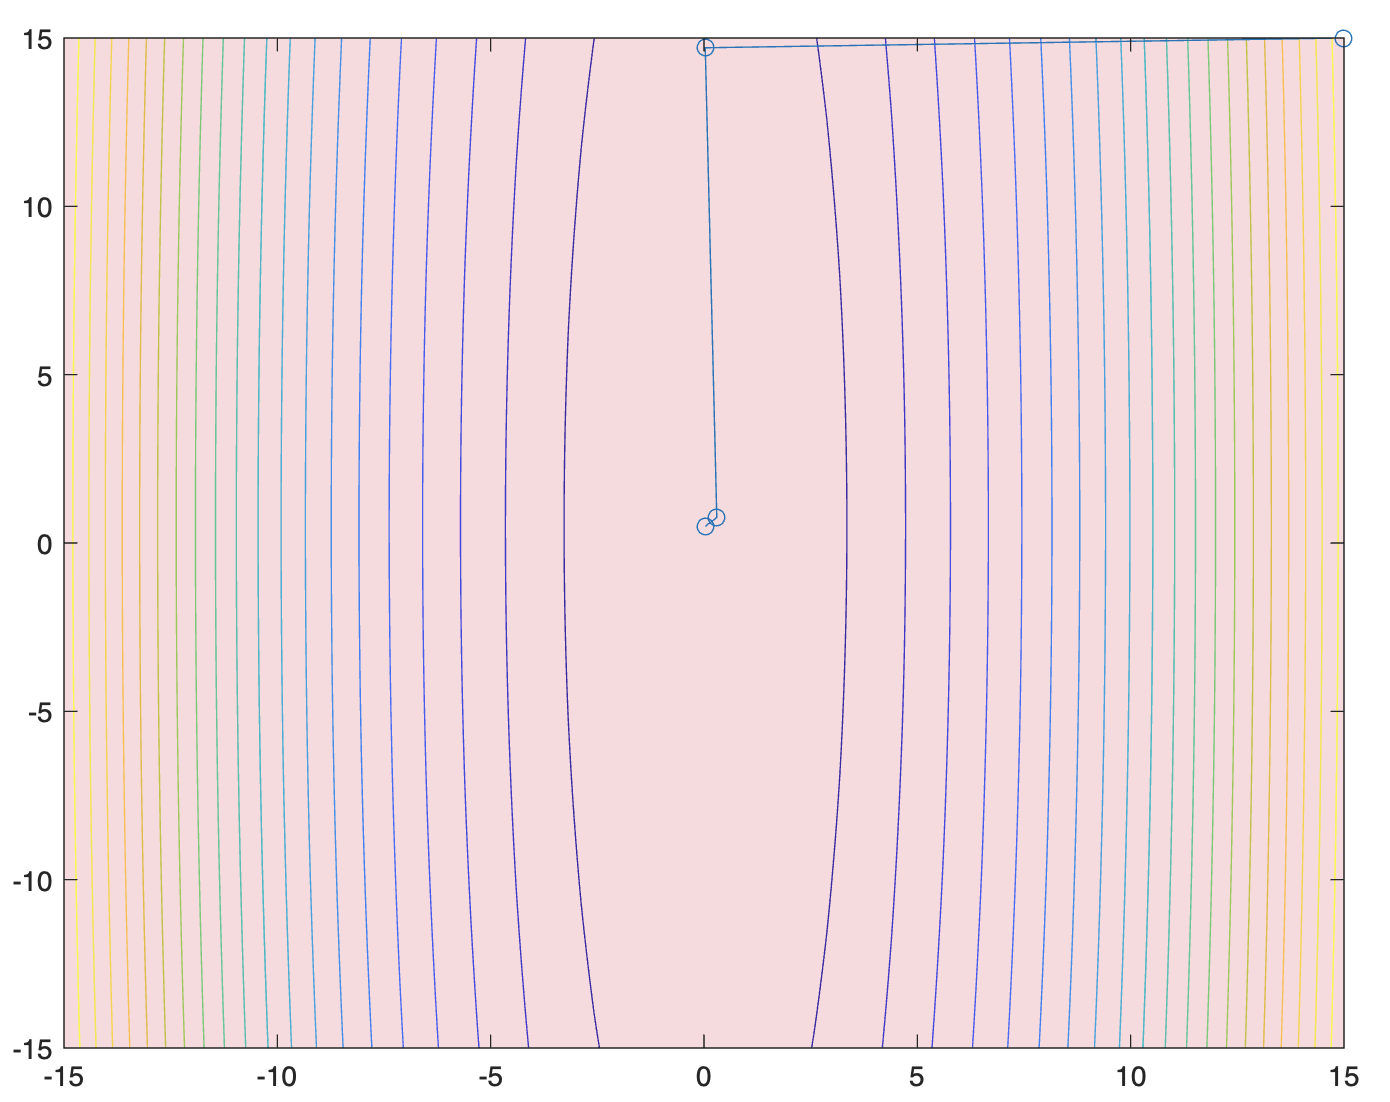
\includegraphics[width=80mm]{p32.png}
\end{center}

Как мы видим, у метода градиентного спуска зигзагообразная траектория. Также в случае овражных функций обычные градиентные методы сходятся плохо. После быстрого спуска в окрестность точки минимума метод начинает медленное движение.

\section{Исследование зависимости числа итераций от размерности пространства и числа обусловленности}

\subsection{Метод Градиентного Спуска}

\begin{figure}[h]
\center{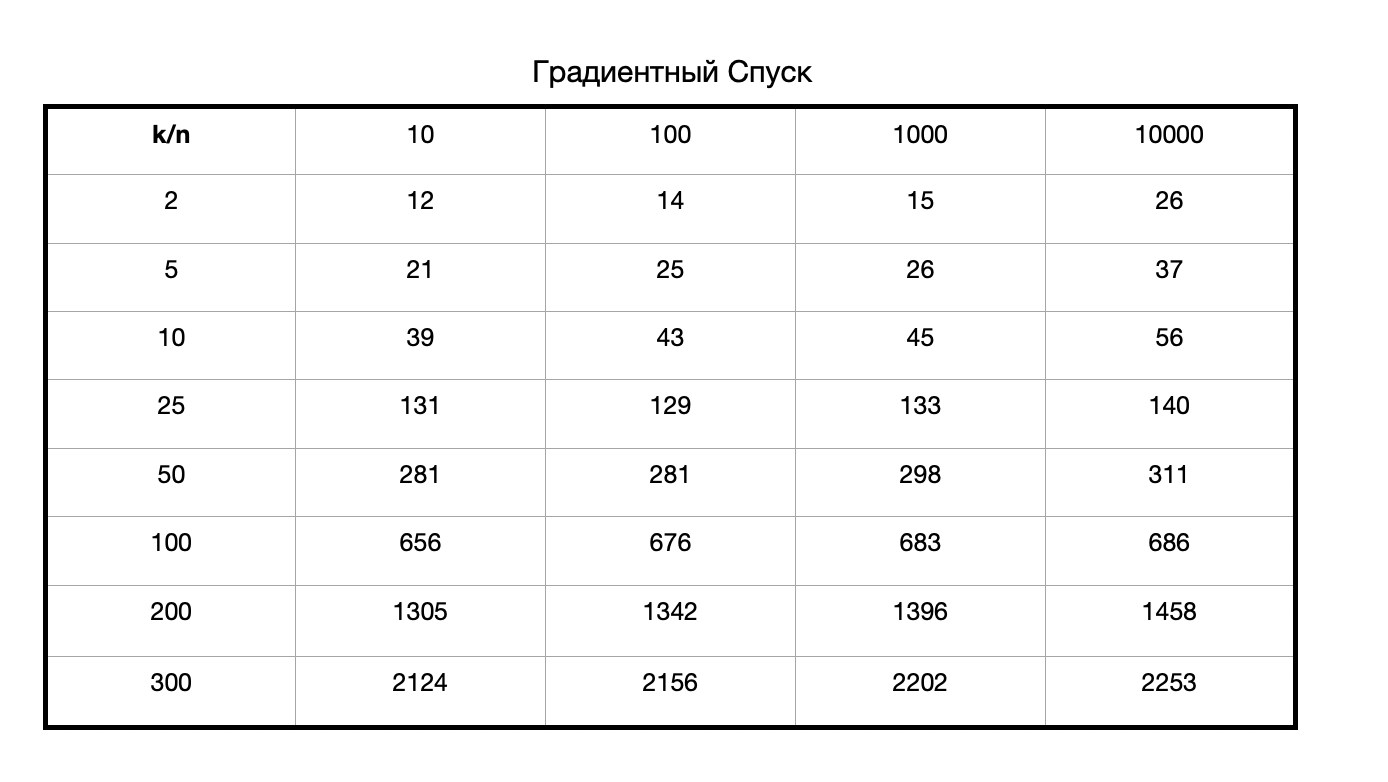
\includegraphics[width=100mm]{descent_table.png}}
\center{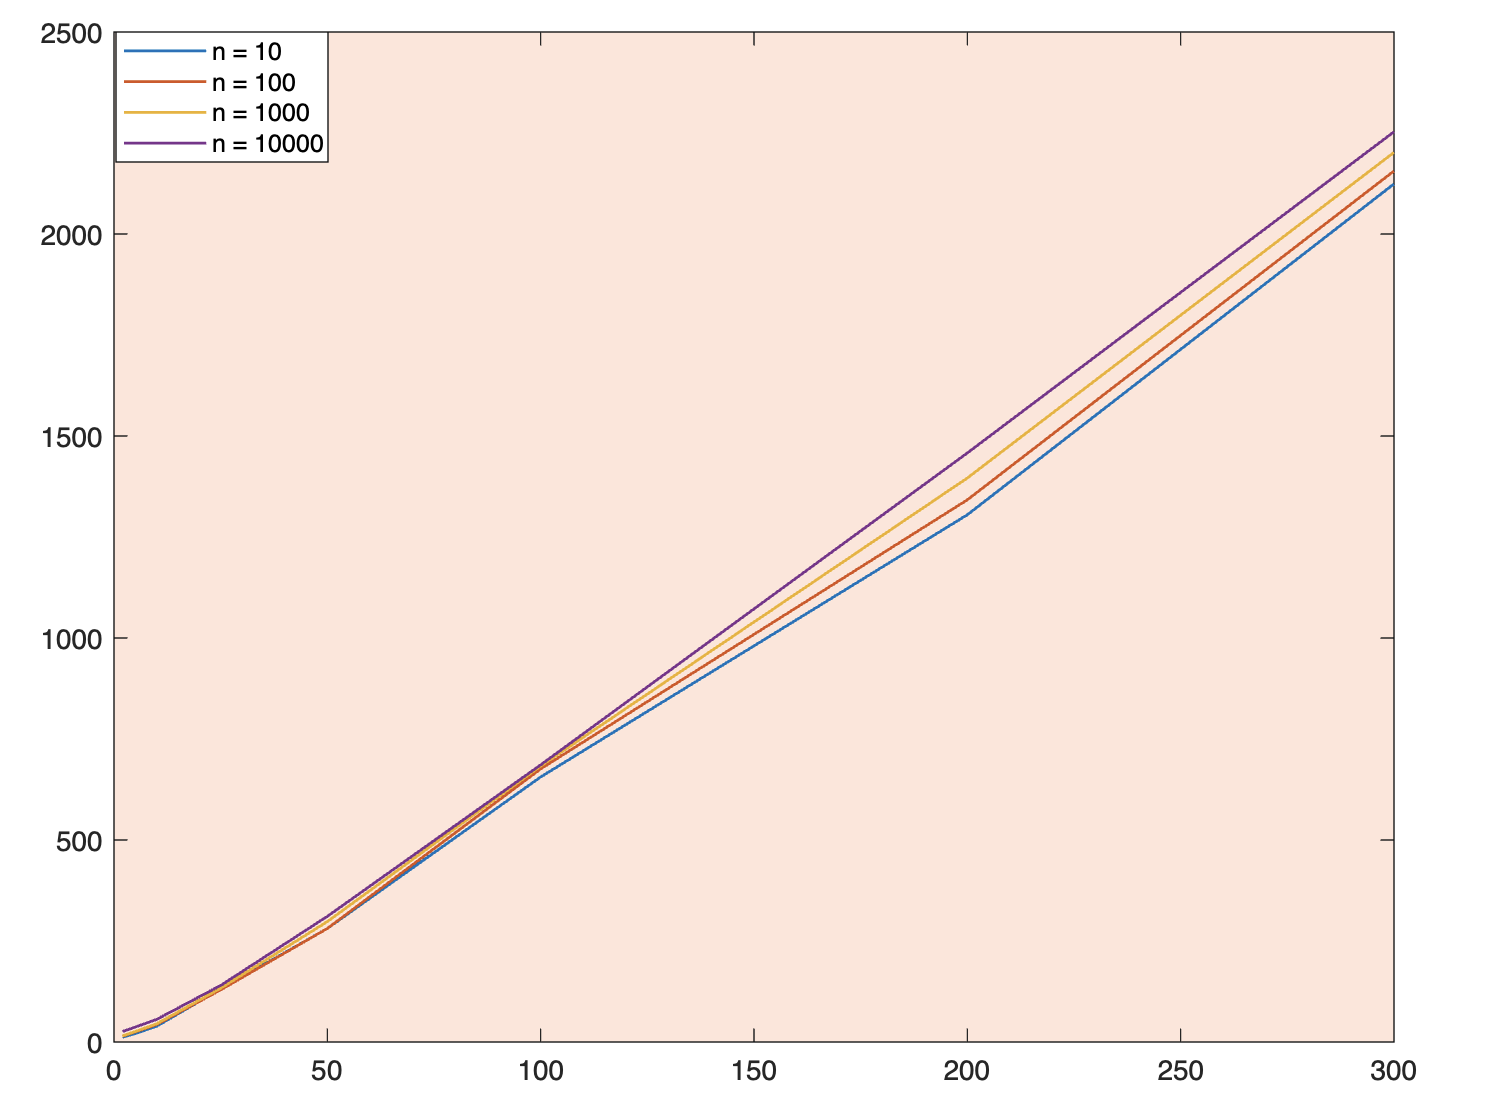
\includegraphics[width=115mm]{descent_plot.png}}
\caption{У МГС число итераций линейно зависит от числа обусловленности и не зависит от размерности.}
\end{figure}

\clearpage

\subsection{Метод Наискорейшего Спуска}

\begin{figure}[h]
\center{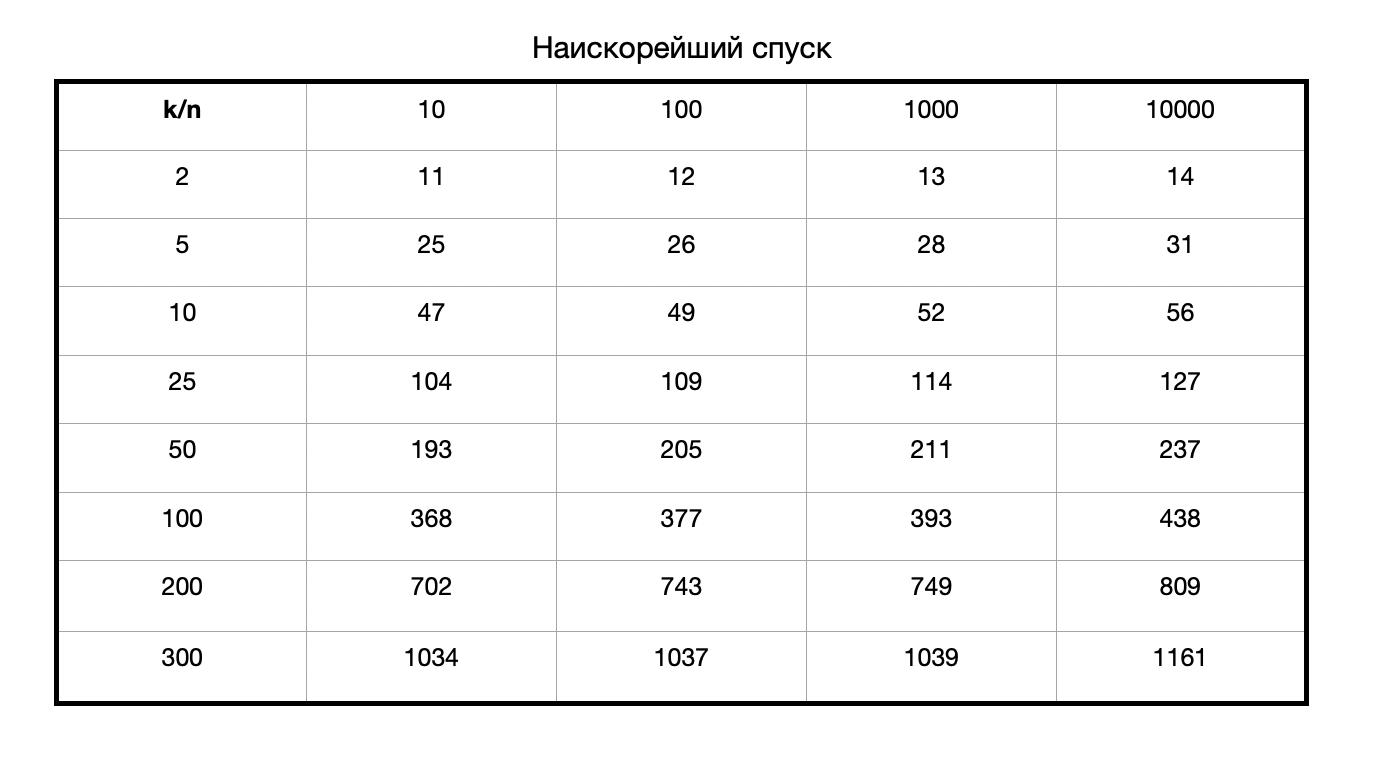
\includegraphics[width=110mm]{fastest_table.png}}
\center{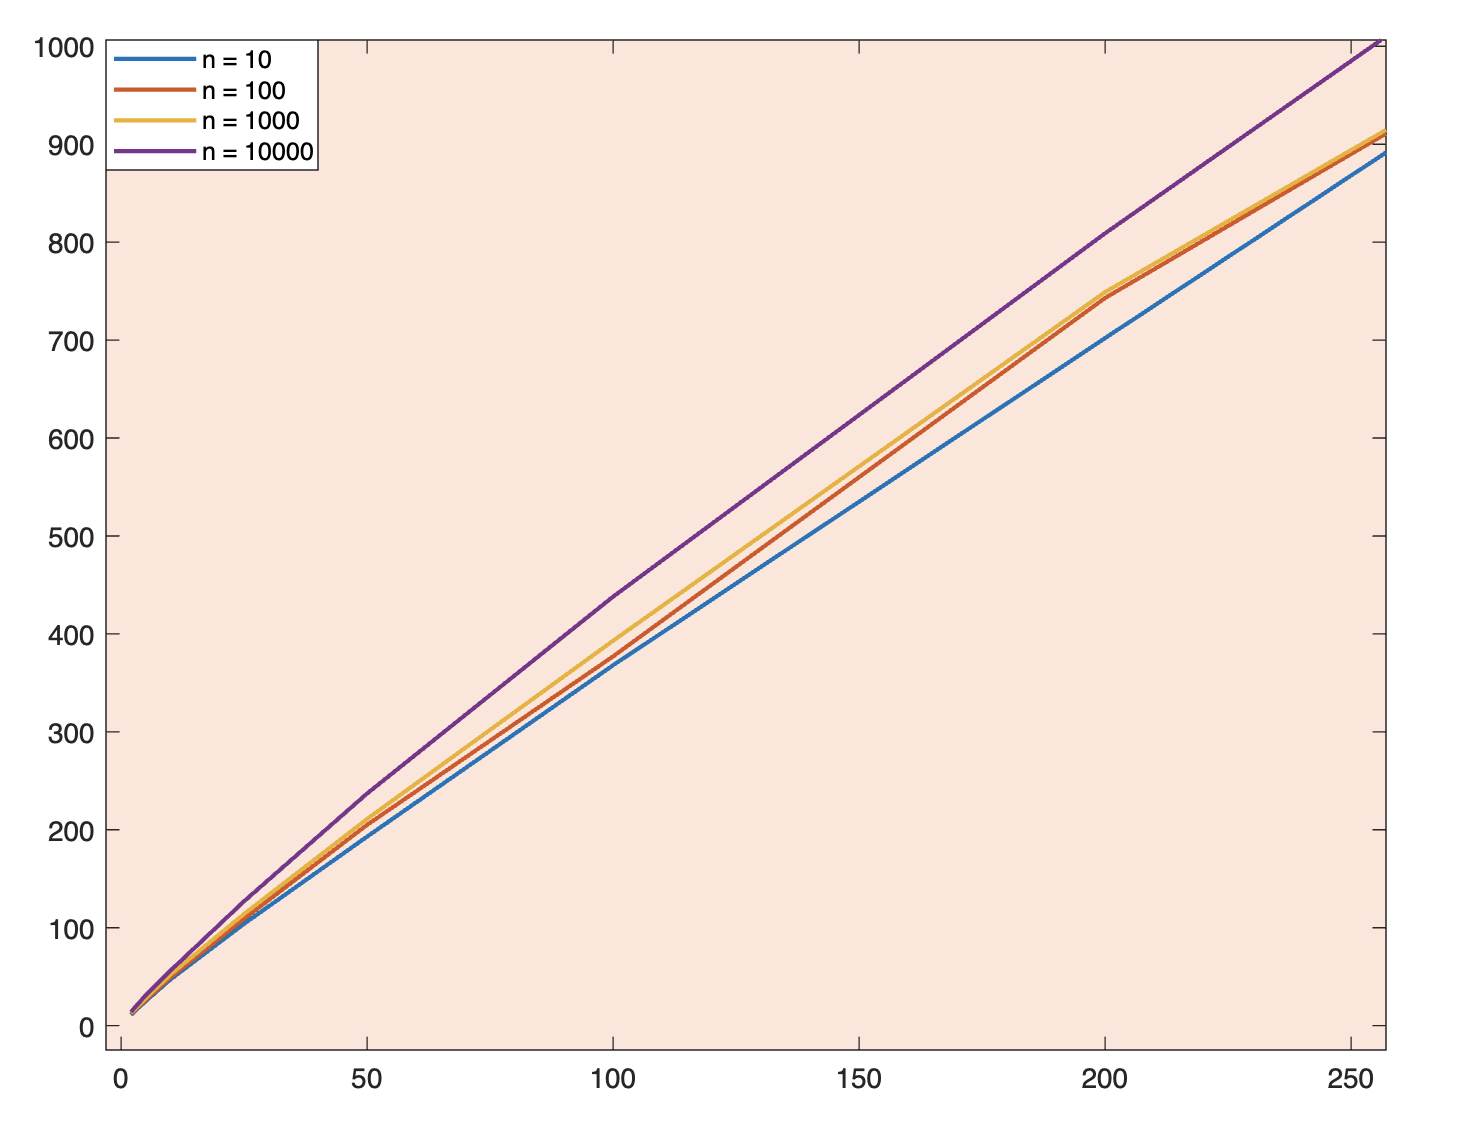
\includegraphics[width=100mm]{fastest_plot.png}}
\caption{МНС делает меньше итераций, чем  МГС, но также как и у последнего число итераций линейно зависит от числа обусловленности и не зависит от размерности.}
\end{figure}

\clearpage

\subsection{Метод Сопряженных Градиентов}

\begin{figure}[h]
\center{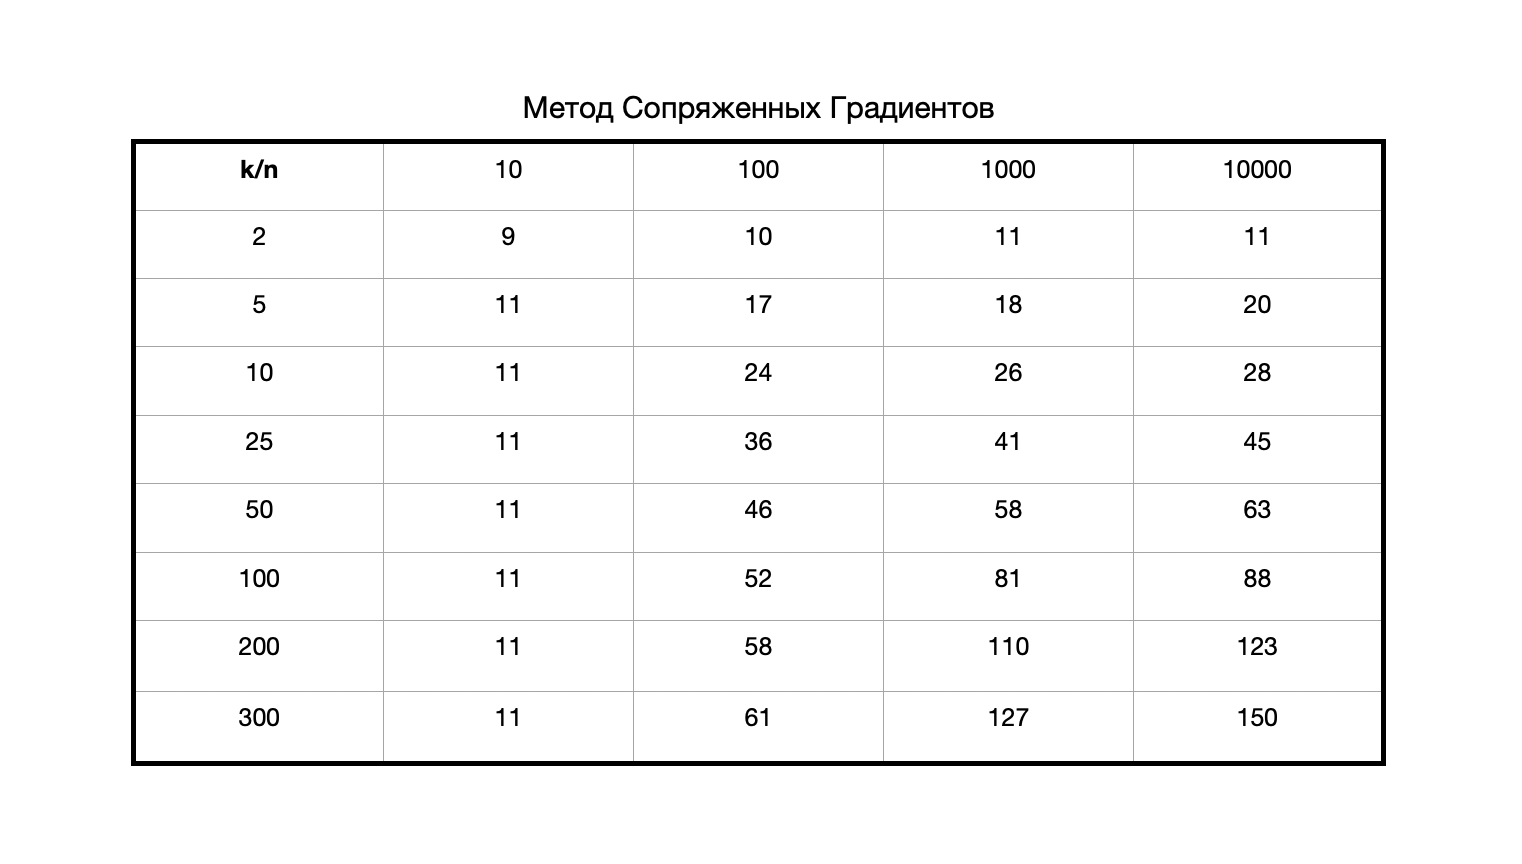
\includegraphics[width=105mm]{conjugate_table.png}}
\center{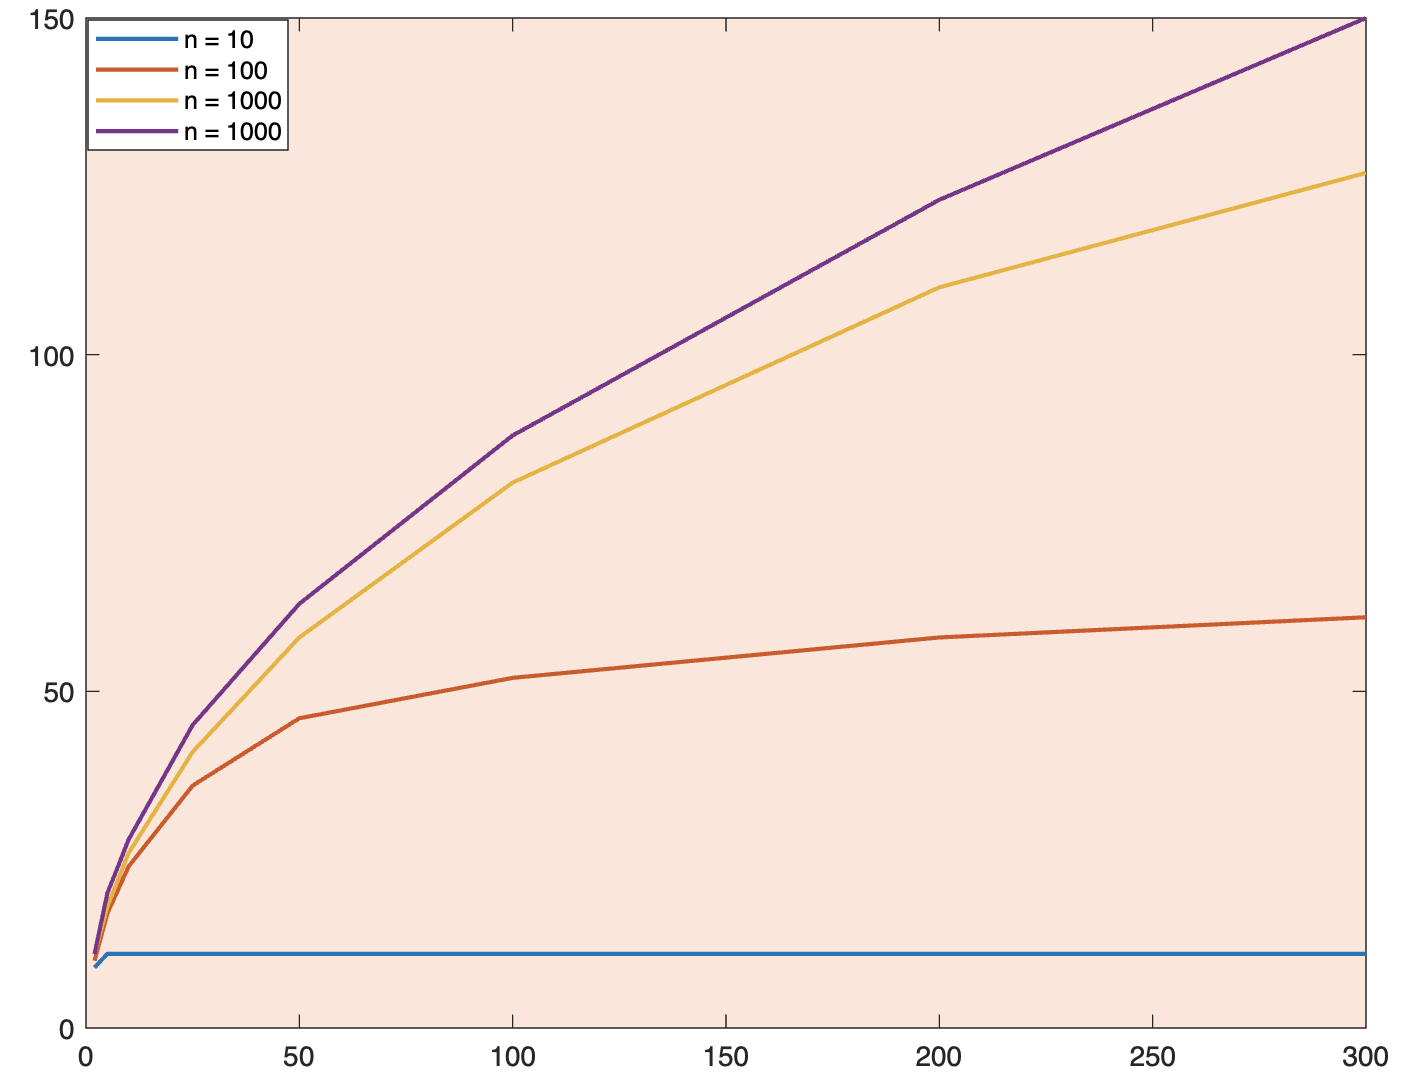
\includegraphics[width=100mm]{conjugate_plot.png}}
\caption{МСГ не зависит от размерности и имеет корневую зависимость от числа обусловленности.}
\end{figure}

\clearpage

\section{Выводы}

\subsection{Траектория}

У метода градиентого спуска зигзагообразная траектория, из чего и вытекает существенное различие в числе итераций с методами наискорейшего спуска и сопряженных градиентов, которые, в свою очередь выстраивают достаточно оптимальную траекторию.

\subsection{Зависимость числа итераций от числа обусловленности и размерности пространства.}

Исходя из графика, видим, что метод градиетного спуска линейно зависит от числа обусловленности. 

Число итераций метода сопряженных градиентов не больше размерности пространства. Также можем заметить, что только у этого метода есть верхняя граница числа итераций при фиксированной размерности.

\subsection{Скорость сходимости}
Выбор одномерного метода оптимизации практически не влияет на количество итераций метода наискорейшего спуска.
\end{document}